\documentclass{article}

\usepackage{amsmath}
\usepackage{tikz}
\usepackage{float}
\usepackage{wasysym}

\usepackage{caption}
\usepackage{subcaption}
\usepackage{fontawesome}
\usepackage{pythonhighlight}
\usepackage{hyperref}
% \usetikzlibrary{automata,arrows,positioning,calc}

\renewcommand{\thesubsection}{\thesection.\alph{subsection}}
\newcommand{\quotes}[1]{``#1''}

\usepackage[]{algorithm2e}

\title{
    \textbf{Estruturas de Dados II}\\
    Algoritmos Elementares em Grafos - VI
}
\author{
    Augusto Emerson\\
    Felipe Monteiro\\
    Jaime Silva\\
    João Victor\\
    Nil Wakya Wai Wai\\
    Sandyella Soares 
}
\date{} % Remova a data

\begin{document}

\begin{titlepage}
    \maketitle
    \thispagestyle{empty}  
\end{titlepage}

\section{} % 1
    A busca em largura (ou Breadth-First Search - BFS) é um algoritmo para percorrer ou buscar em um grafo. A característica principal da BFS é que ela explora todos os vizinhos de um vértice antes de passar para os vizinhos dos vizinhos.
     
    Os vértices a serem visitados são colocadas em uma fila, inicialmente apenas com o vértice inicial. Na medida que visitamos os adjacentes desse vértice, ele é adicionado na fila apenas se não estiverem na fila, os vértices já visitados, mas que os adjacentes são desconhecidos o vértice é pintado de cinza, os vértices já visitados e os adjacentes visitados são pintados de preto e removidos da fila. Se a fila estiver vazia e ainda restarem vértices não visitados, reiniciamos o procedimento a partir desses vértices.\\
    
    \indent{Defina uma inicial, marcado como explorada}\\
    \indent{Enfileire-os na fila}\\
    \indent{Enquanto a fila não estiver vazia:}\\
    \indent\indent{Remova o primeiro vértice da fila $u$}\\
    \indent\indent{Para cada vizinho $v$ de $u$:}\\
    \indent\indent\indent{Se $v$ não explorado:}\\
    \indent\indent\indent\indent{Marque $v$ como explorado}\\
    \indent\indent\indent\indent{E coloque $v$ no fim da fila}\\
    \indent{Repita de outro vértice inicial, se houver}

\section{} % 2
    \begin{figure}[H]
        \centering
        \begin{subfigure}{0.30\textwidth}
            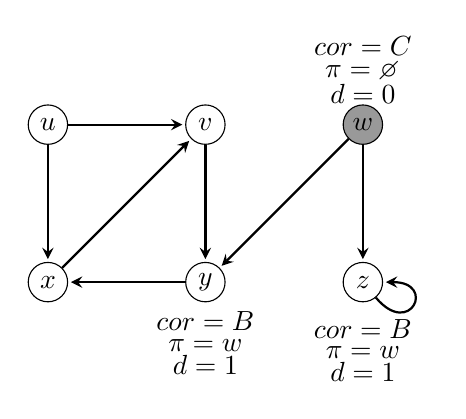
\begin{tikzpicture}[> = stealth,  shorten > = 1pt,   auto,   node distance = 1.5cm]
                \tikzstyle{vertex}=[circle, draw, inner sep=0pt, minimum size=5mm]
                    % Nós
                    \node[vertex] (u) at (0,0) {$u$};
                    \node[vertex] (x) at (0,-2) {$x$};
                    \node[vertex] (v) at (2,0) {$v$};
                    \node[vertex] (y) at (2,-2) {$y$};
                    \node[vertex, fill=gray!80] (w) at (4,0) {$w$};
                    \node[vertex] (z) at (4,-2) {$z$};

                    % Arestas
                    \draw[->,thick] (u) -- (x);
                    \draw[->,thick] (u) -- (v);
                    \draw[->,thick] (x) -- (v);
                    \draw[->,thick] (v) -- (y);
                    \draw[->,thick] (y) -- (x);
                    \draw[->,thick] (w) -- (y);
                    \draw[->,thick] (w) -- (z);
                    \draw[->,thick] (z) to [out=-50,in=0,looseness=8] (z);

                    % Anotações
                    \node at (w) [above=.75cm] {$cor = C$};
                    \node at (w) [above=.45cm] {$\pi = \diameter$};
                    \node at (w) [above=.15cm] {$d = 0$};
                    
                    \node at (z) [below=.35cm] {$cor = B$};
                    \node at (z) [below=.7cm] {$\pi = w$};
                    \node at (z) [below=.9cm] {$d = 1$};

                    \node at (y) [below=.25cm] {$cor = B$};
                    \node at (y) [below=.6cm] {$\pi = w$};
                    \node at (y) [below=.8cm] {$d = 1$};

                \end{tikzpicture}
            \caption{}
        \end{subfigure}
    \end{figure}
    \clearpage
    \begin{figure}[H]\ContinuedFloat
        \centering
        \begin{subfigure}{0.30\textwidth}
            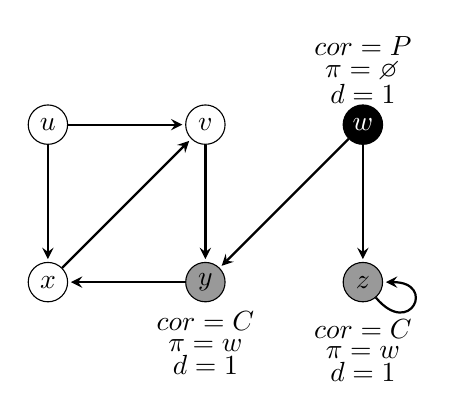
\begin{tikzpicture}[> = stealth,  shorten > = 1pt,   auto,   node distance = 1.5cm]
                \tikzstyle{vertex}=[circle, draw, inner sep=0pt, minimum size=5mm]
                    % Nós
                    \node[vertex] (u) at (0,0) {$u$};
                    \node[vertex] (x) at (0,-2) {$x$};
                    \node[vertex] (v) at (2,0) {$v$};
                    \node[vertex, fill=gray!80] (y) at (2,-2) {$y$};
                    \node[vertex, fill=black, text=white] (w) at (4,0) {$w$};
                    \node[vertex, fill=gray!80] (z) at (4,-2) {$z$};

                    % Arestas
                    \draw[->,thick] (u) -- (x);
                    \draw[->,thick] (u) -- (v);
                    \draw[->,thick] (x) -- (v);
                    \draw[->,thick] (v) -- (y);
                    \draw[->,thick] (y) -- (x);
                    \draw[->,thick] (w) -- (y);
                    \draw[->,thick] (w) -- (z);
                    \draw[->,thick] (z) to [out=-50,in=0,looseness=8] (z);

                    % Anotações
                    \node at (y) [below=.25cm] {$cor = C$};
                    \node at (y) [below=.6cm] {$\pi = w$};
                    \node at (y) [below=.8cm] {$d = 1$};

                    \node at (z) [below=.35cm] {$cor = C$};
                    \node at (z) [below=.7cm] {$\pi = w$};
                    \node at (z) [below=.9cm] {$d = 1$};

                    \node at (w) [above=.75cm] {$cor = P$};
                    \node at (w) [above=.45cm] {$\pi = \diameter$};
                    \node at (w) [above=.15cm] {$d = 1$};

                \end{tikzpicture}
            \caption{}
        \end{subfigure}
        \\
        \begin{subfigure}{0.30\textwidth}
            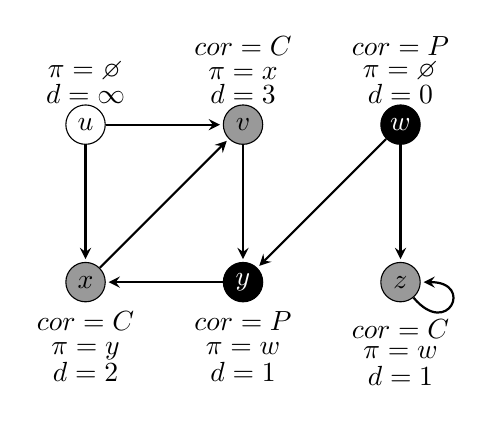
\begin{tikzpicture}[> = stealth,  shorten > = 1pt,   auto,   node distance = 1.5cm]
                \tikzstyle{vertex}=[circle, draw, inner sep=0pt, minimum size=5mm]
                    % Nós
                    \node[vertex] (u) at (0,0) {$u$};
                    \node[vertex, fill=gray!80] (x) at (0,-2) {$x$};
                    \node[vertex, fill=gray!80] (v) at (2,0) {$v$};
                    \node[vertex, fill=black, text=white] (y) at (2,-2) {$y$};
                    \node[vertex, fill=black, text=white] (w) at (4,0) {$w$};
                    \node[vertex, fill=gray!80] (z) at (4,-2) {$z$};

                    % Arestas
                    \draw[->,thick] (u) -- (x);
                    \draw[->,thick] (u) -- (v);
                    \draw[->,thick] (x) -- (v);
                    \draw[->,thick] (v) -- (y);
                    \draw[->,thick] (y) -- (x);
                    \draw[->,thick] (w) -- (y);
                    \draw[->,thick] (w) -- (z);
                    \draw[->,thick] (z) to [out=-50,in=0,looseness=8] (z);

                    % Anotações
                    \node at (y) [below=.25cm] {$cor = P$};
                    \node at (y) [below=.65cm] {$\pi = w$};
                    \node at (y) [below=.9cm] {$d = 1$};

                    \node at (z) [below=.35cm] {$cor = C$};
                    \node at (z) [below=.7cm] {$\pi = w$};
                    \node at (z) [below=.95cm] {$d = 1$};
                    
                    \node at (v) [above=.75cm] {$cor = C$};
                    \node at (v) [above=.45cm] {$\pi = x$};
                    \node at (v) [above=.15cm] {$d = 3$};
                    
                    \node at (x) [below=.25cm] {$cor = C$};
                    \node at (x) [below=.65cm] {$\pi = y$};
                    \node at (x) [below=.9cm] {$d = 2$};

                    \node at (w) [above=.75cm] {$cor = P$};
                    \node at (w) [above=.45cm] {$\pi = \diameter$};
                    \node at (w) [above=.15cm] {$d = 0$};

                    \node at (u) [above=.45cm] {$\pi = \diameter$};
                    \node at (u) [above=.15cm] {$d = \infty$};

                \end{tikzpicture}
            \caption{}
        \end{subfigure}
        \\
        \begin{subfigure}{0.30\textwidth}
            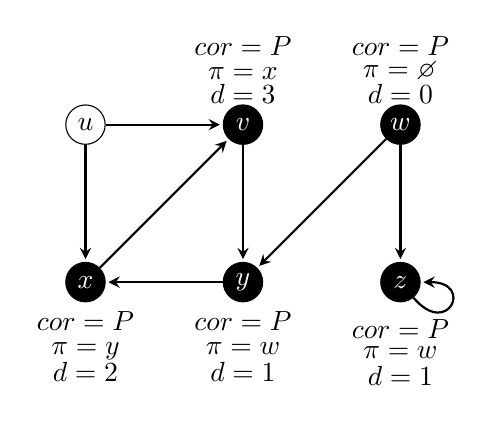
\begin{tikzpicture}[> = stealth,  shorten > = 1pt,   auto,   node distance = 1.5cm]
                \tikzstyle{vertex}=[circle, draw, inner sep=0pt, minimum size=5mm]
                    % Nós
                    \node[vertex] (u) at (0,0) {$u$};
                    \node[vertex, fill=black, text=white] (x) at (0,-2) {$x$};
                    \node[vertex, fill=black, text=white] (v) at (2,0) {$v$};
                    \node[vertex, fill=black, text=white] (y) at (2,-2) {$y$};
                    \node[vertex, fill=black, text=white] (w) at (4,0) {$w$};
                    \node[vertex, fill=black, text=white] (z) at (4,-2) {$z$};

                    % Arestas
                    \draw[->,thick] (u) -- (x);
                    \draw[->,thick] (u) -- (v);
                    \draw[->,thick] (x) -- (v);
                    \draw[->,thick] (v) -- (y);
                    \draw[->,thick] (y) -- (x);
                    \draw[->,thick] (w) -- (y);
                    \draw[->,thick] (w) -- (z);
                    \draw[->,thick] (z) to [out=-50,in=0,looseness=8] (z);

                    % Anotações
                    \node at (y) [below=.25cm] {$cor = P$};
                    \node at (y) [below=.65cm] {$\pi = w$};
                    \node at (y) [below=.9cm] {$d = 1$};

                    \node at (z) [below=.35cm] {$cor = P$};
                    \node at (z) [below=.7cm] {$\pi = w$};
                    \node at (z) [below=.95cm] {$d = 1$};
                    
                    \node at (v) [above=.75cm] {$cor = P$};
                    \node at (v) [above=.45cm] {$\pi = x$};
                    \node at (v) [above=.15cm] {$d = 3$};
                    
                    \node at (x) [below=.25cm] {$cor = P$};
                    \node at (x) [below=.65cm] {$\pi = y$};
                    \node at (x) [below=.9cm] {$d = 2$};

                    \node at (w) [above=.75cm] {$cor = P$};
                    \node at (w) [above=.45cm] {$\pi = \diameter$};
                    \node at (w) [above=.15cm] {$d = 0$};

                \end{tikzpicture}
            \caption{}
        \end{subfigure}
    \end{figure}

\section{} % 3

    \begin{figure}[H]
        \begin{subfigure}{\textwidth}
            \centering
            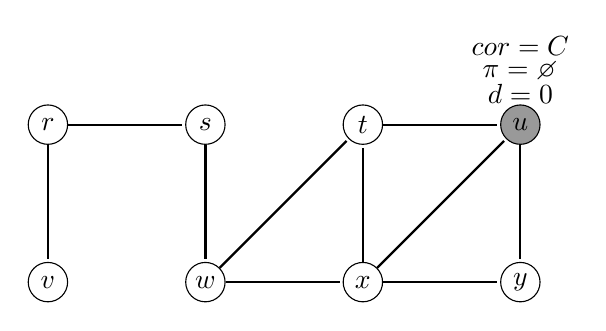
\begin{tikzpicture}[> = stealth,  shorten > = 1pt,   auto,   node distance = 1.5cm]
                \tikzstyle{vertex}=[circle, draw, inner sep=0pt, minimum size=5mm]
        
                    % Nós
                    \node[vertex] (r) at (0,0) {$r$};
                    \node[vertex] (s) at (2,0) {$s$};
                    \node[vertex] (t) at (4,0) {$t$};
                    \node[vertex, fill=gray!80] (u) at (6,0) {$u$};
                    \node[vertex] (v) at (0,-2) {$v$};
                    \node[vertex] (w) at (2,-2) {$w$};
                    \node[vertex] (x) at (4,-2) {$x$};
                    \node[vertex] (y) at (6,-2) {$y$};
                    
                    % Arestas
                    \draw[-,thick] (r) -- (v);
                    \draw[-,thick] (r) -- (s);
                    \draw[-,thick] (s) -- (w);
                    \draw[-,thick] (w) -- (t);
                    \draw[-,thick] (w) -- (x);
                    \draw[-,thick] (x) -- (y);
                    \draw[-,thick] (x) -- (u);
                    \draw[-,thick] (x) -- (t);
                    \draw[-,thick] (t) -- (u);
                    \draw[-,thick] (u) -- (y);

                    \node at (u) [above=.75cm] {$cor = C$};
                    \node at (u) [above=.45cm] {$\pi = \diameter$};
                    \node at (u) [above=.15cm] {$d = 0$};
            \end{tikzpicture}
            \caption{}
        \end{subfigure}
        \\

        \begin{subfigure}{\textwidth}
            \centering
            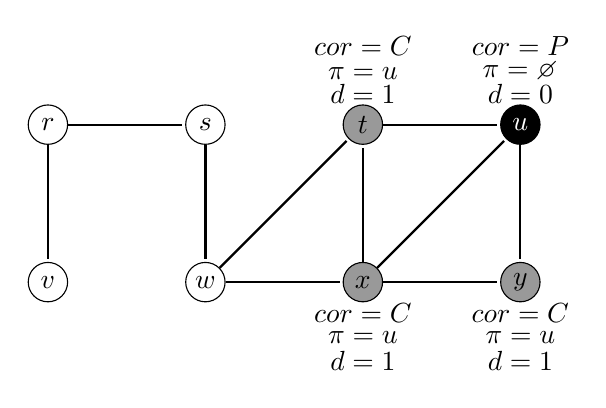
\begin{tikzpicture}[> = stealth,  shorten > = 1pt,   auto,   node distance = 1.5cm]
                \tikzstyle{vertex}=[circle, draw, inner sep=0pt, minimum size=5mm]
        
                    % Nós
                    \node[vertex] (r) at (0,0) {$r$};
                    \node[vertex] (s) at (2,0) {$s$};
                    \node[vertex, fill=gray!80] (t) at (4,0) {$t$};
                    \node[vertex, fill=black, text=white] (u) at (6,0) {$u$};
                    \node[vertex] (v) at (0,-2) {$v$};
                    \node[vertex] (w) at (2,-2) {$w$};
                    \node[vertex, fill=gray!80] (x) at (4,-2) {$x$};
                    \node[vertex, fill=gray!80] (y) at (6,-2) {$y$};
                    
                    % Arestas
                    \draw[-,thick] (r) -- (v);
                    \draw[-,thick] (r) -- (s);
                    \draw[-,thick] (s) -- (w);
                    \draw[-,thick] (w) -- (t);
                    \draw[-,thick] (w) -- (x);
                    \draw[-,thick] (x) -- (y);
                    \draw[-,thick] (x) -- (u);
                    \draw[-,thick] (x) -- (t);
                    \draw[-,thick] (t) -- (u);
                    \draw[-,thick] (u) -- (y);

                    \node at (u) [above=.75cm] {$cor = P$};
                    \node at (u) [above=.45cm] {$\pi = \diameter$};
                    \node at (u) [above=.15cm] {$d = 0$}; 
                    
                    \node at (t) [above=.75cm] {$cor = C$};
                    \node at (t) [above=.45cm] {$\pi = u$};
                    \node at (t) [above=.15cm] {$d = 1$};

                    \node at (x) [below=.15cm] {$cor = C$};
                    \node at (x) [below=.5cm] {$\pi = u$};
                    \node at (x) [below=.75cm] {$d = 1$};
                    
                    \node at (y) [below=.15cm] {$cor = C$};
                    \node at (y) [below=.5cm] {$\pi = u$};
                    \node at (y) [below=.75cm] {$d = 1$};
            \end{tikzpicture}
            \caption{}
        \end{subfigure}
        \\

        \begin{subfigure}{\textwidth}
            \centering
            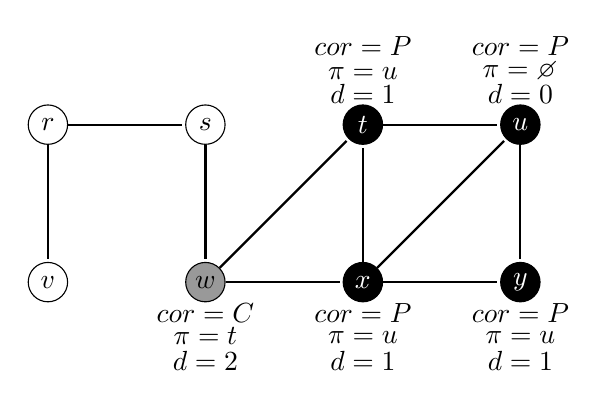
\begin{tikzpicture}[> = stealth,  shorten > = 1pt,   auto,   node distance = 1.5cm]
                \tikzstyle{vertex}=[circle, draw, inner sep=0pt, minimum size=5mm]
        
                    % Nós
                    \node[vertex] (r) at (0,0) {$r$};
                    \node[vertex] (s) at (2,0) {$s$};
                    \node[vertex, fill=black, text=white] (t) at (4,0) {$t$};
                    \node[vertex, fill=black, text=white] (u) at (6,0) {$u$};
                    \node[vertex] (v) at (0,-2) {$v$};
                    \node[vertex, fill=gray!80] (w) at (2,-2) {$w$};
                    \node[vertex, fill=black, text=white] (x) at (4,-2) {$x$};
                    \node[vertex, fill=black, text=white] (y) at (6,-2) {$y$};
                    
                    % Arestas
                    \draw[-,thick] (r) -- (v);
                    \draw[-,thick] (r) -- (s);
                    \draw[-,thick] (s) -- (w);
                    \draw[-,thick] (w) -- (t);
                    \draw[-,thick] (w) -- (x);
                    \draw[-,thick] (x) -- (y);
                    \draw[-,thick] (x) -- (u);
                    \draw[-,thick] (x) -- (t);
                    \draw[-,thick] (t) -- (u);
                    \draw[-,thick] (u) -- (y);

                    \node at (u) [above=.75cm] {$cor = P$};
                    \node at (u) [above=.45cm] {$\pi = \diameter$};
                    \node at (u) [above=.15cm] {$d = 0$}; 
                    
                    \node at (t) [above=.75cm] {$cor = P$};
                    \node at (t) [above=.45cm] {$\pi = u$};
                    \node at (t) [above=.15cm] {$d = 1$};

                    \node at (x) [below=.15cm] {$cor = P$};
                    \node at (x) [below=.5cm] {$\pi = u$};
                    \node at (x) [below=.75cm] {$d = 1$};
                    
                    \node at (y) [below=.15cm] {$cor = P$};
                    \node at (y) [below=.5cm] {$\pi = u$};
                    \node at (y) [below=.75cm] {$d = 1$};

                    \node at (w) [below=.15cm] {$cor = C$};
                    \node at (w) [below=.45cm] {$\pi = t$};
                    \node at (w) [below=.75cm] {$d = 2$};
            \end{tikzpicture}
            \caption{}
        \end{subfigure}

    \end{figure}
    \clearpage
    \begin{figure}[H]\ContinuedFloat

        \begin{subfigure}{\textwidth}
            \centering
            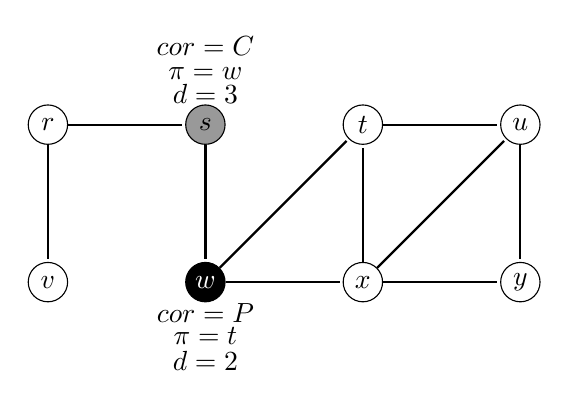
\begin{tikzpicture}[> = stealth,  shorten > = 1pt,   auto,   node distance = 1.5cm]
                \tikzstyle{vertex}=[circle, draw, inner sep=0pt, minimum size=5mm]
        
                    % Nós
                    \node[vertex] (r) at (0,0) {$r$};
                    \node[vertex, fill=gray!80] (s) at (2,0) {$s$};
                    \node[vertex] (t) at (4,0) {$t$};
                    \node[vertex] (u) at (6,0) {$u$};
                    \node[vertex] (v) at (0,-2) {$v$};
                    \node[vertex, fill=black, text=white] (w) at (2,-2) {$w$};
                    \node[vertex] (x) at (4,-2) {$x$};
                    \node[vertex] (y) at (6,-2) {$y$};
                    
                    % Arestas
                    \draw[-,thick] (r) -- (v);
                    \draw[-,thick] (r) -- (s);
                    \draw[-,thick] (s) -- (w);
                    \draw[-,thick] (w) -- (t);
                    \draw[-,thick] (w) -- (x);
                    \draw[-,thick] (x) -- (y);
                    \draw[-,thick] (x) -- (u);
                    \draw[-,thick] (x) -- (t);
                    \draw[-,thick] (t) -- (u);
                    \draw[-,thick] (u) -- (y);

                    \node at (s) [above=.75cm] {$cor = C$};
                    \node at (s) [above=.45cm] {$\pi = w$};
                    \node at (s) [above=.15cm] {$d = 3$};

                    \node at (w) [below=.15cm] {$cor = P$};
                    \node at (w) [below=.45cm] {$\pi = t$};
                    \node at (w) [below=.75cm] {$d = 2$};
            \end{tikzpicture}
            \caption{}
        \end{subfigure}
        \\
    
        \begin{subfigure}{\textwidth}
            \centering
            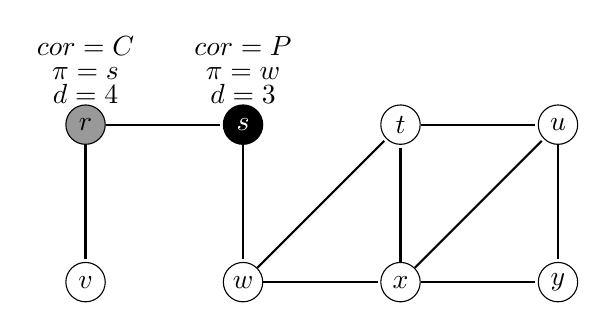
\begin{tikzpicture}[> = stealth,  shorten > = 1pt,   auto,   node distance = 1.5cm]
                \tikzstyle{vertex}=[circle, draw, inner sep=0pt, minimum size=5mm]
        
                    % Nós
                    \node[vertex, fill=gray!80] (r) at (0,0) {$r$};
                    \node[vertex, fill=black, text=white] (s) at (2,0) {$s$};
                    \node[vertex] (t) at (4,0) {$t$};
                    \node[vertex] (u) at (6,0) {$u$};
                    \node[vertex] (v) at (0,-2) {$v$};
                    \node[vertex] (w) at (2,-2) {$w$};
                    \node[vertex] (x) at (4,-2) {$x$};
                    \node[vertex] (y) at (6,-2) {$y$};
                    
                    % Arestas
                    \draw[-,thick] (r) -- (v);
                    \draw[-,thick] (r) -- (s);
                    \draw[-,thick] (s) -- (w);
                    \draw[-,thick] (w) -- (t);
                    \draw[-,thick] (w) -- (x);
                    \draw[-,thick] (x) -- (y);
                    \draw[-,thick] (x) -- (u);
                    \draw[-,thick] (x) -- (t);
                    \draw[-,thick] (t) -- (u);
                    \draw[-,thick] (u) -- (y);
                    
                    \node at (r) [above=.75cm] {$cor = C$};
                    \node at (r) [above=.45cm] {$\pi = s$};
                    \node at (r) [above=.15cm] {$d = 4$};
                    
                    \node at (s) [above=.75cm] {$cor = P$};
                    \node at (s) [above=.45cm] {$\pi = w$};
                    \node at (s) [above=.15cm] {$d = 3$};
            \end{tikzpicture}
            \caption{}
        \end{subfigure}
        \\

        \begin{subfigure}{\textwidth}
            \centering
            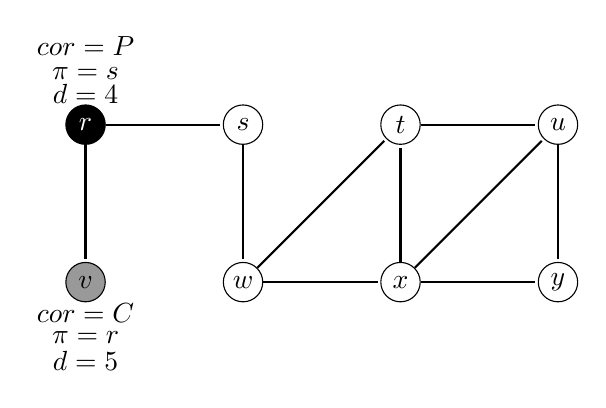
\begin{tikzpicture}[> = stealth,  shorten > = 1pt,   auto,   node distance = 1.5cm]
                \tikzstyle{vertex}=[circle, draw, inner sep=0pt, minimum size=5mm]
        
                    % Nós
                    \node[vertex, fill=black, text=white] (r) at (0,0) {$r$};
                    \node[vertex] (s) at (2,0) {$s$};
                    \node[vertex] (t) at (4,0) {$t$};
                    \node[vertex] (u) at (6,0) {$u$};
                    \node[vertex, fill=gray!80] (v) at (0,-2) {$v$};
                    \node[vertex] (w) at (2,-2) {$w$};
                    \node[vertex] (x) at (4,-2) {$x$};
                    \node[vertex] (y) at (6,-2) {$y$};
                    
                    % Arestas
                    \draw[-,thick] (r) -- (v);
                    \draw[-,thick] (r) -- (s);
                    \draw[-,thick] (s) -- (w);
                    \draw[-,thick] (w) -- (t);
                    \draw[-,thick] (w) -- (x);
                    \draw[-,thick] (x) -- (y);
                    \draw[-,thick] (x) -- (u);
                    \draw[-,thick] (x) -- (t);
                    \draw[-,thick] (t) -- (u);
                    \draw[-,thick] (u) -- (y);
                    
                    \node at (r) [above=.75cm] {$cor = P$};
                    \node at (r) [above=.45cm] {$\pi = s$};
                    \node at (r) [above=.15cm] {$d = 4$};

                    \node at (v) [below=.15cm] {$cor = C$};
                    \node at (v) [below=.5cm] {$\pi = r$};
                    \node at (v) [below=.75cm] {$d = 5$};
                

            \end{tikzpicture}
            \caption{}
        \end{subfigure}

    \end{figure}
    \clearpage
    \begin{figure}[H]\ContinuedFloat

        \begin{subfigure}{\textwidth}
            \centering
            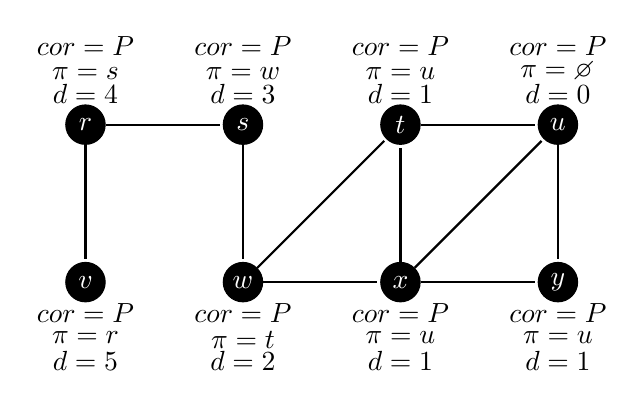
\begin{tikzpicture}[> = stealth,  shorten > = 1pt,   auto,   node distance = 1.5cm]
                \tikzstyle{vertex}=[circle, draw, inner sep=0pt, minimum size=5mm]
        
                    % Nós
                    \node[vertex, fill=black, text=white] (r) at (0,0) {$r$};
                    \node[vertex, fill=black, text=white] (s) at (2,0) {$s$};
                    \node[vertex, fill=black, text=white] (t) at (4,0) {$t$};
                    \node[vertex, fill=black, text=white] (u) at (6,0) {$u$};
                    \node[vertex, fill=black, text=white] (v) at (0,-2) {$v$};
                    \node[vertex, fill=black, text=white] (w) at (2,-2) {$w$};
                    \node[vertex, fill=black, text=white] (x) at (4,-2) {$x$};
                    \node[vertex, fill=black, text=white] (y) at (6,-2) {$y$};
                    
                    % Arestas
                    \draw[-,thick] (r) -- (v);
                    \draw[-,thick] (r) -- (s);
                    \draw[-,thick] (s) -- (w);
                    \draw[-,thick] (w) -- (t);
                    \draw[-,thick] (w) -- (x);
                    \draw[-,thick] (x) -- (y);
                    \draw[-,thick] (x) -- (u);
                    \draw[-,thick] (x) -- (t);
                    \draw[-,thick] (t) -- (u);
                    \draw[-,thick] (u) -- (y);

                    % Anotações
                    \node at (r) [above=.75cm] {$cor = P$};
                    \node at (r) [above=.45cm] {$\pi = s$};
                    \node at (r) [above=.15cm] {$d = 4$};
                    
                    \node at (s) [above=.75cm] {$cor = P$};
                    \node at (s) [above=.45cm] {$\pi = w$};
                    \node at (s) [above=.15cm] {$d = 3$};
                    
                    \node at (t) [above=.75cm] {$cor = P$};
                    \node at (t) [above=.45cm] {$\pi = u$};
                    \node at (t) [above=.15cm] {$d = 1$};
                    
                    \node at (u) [above=.75cm] {$cor = P$};
                    \node at (u) [above=.45cm] {$\pi = \diameter$};
                    \node at (u) [above=.15cm] {$d = 0$};
                    
                    \node at (v) [below=.15cm] {$cor = P$};
                    \node at (v) [below=.5cm] {$\pi = r$};
                    \node at (v) [below=.75cm] {$d = 5$};
                
                    \node at (w) [below=.15cm] {$cor = P$};
                    \node at (w) [below=.5cm] {$\pi = t$};
                    \node at (w) [below=.75cm] {$d = 2$};
                    
                    \node at (x) [below=.15cm] {$cor = P$};
                    \node at (x) [below=.5cm] {$\pi = u$};
                    \node at (x) [below=.75cm] {$d = 1$};
                    
                    \node at (y) [below=.15cm] {$cor = P$};
                    \node at (y) [below=.5cm] {$\pi = u$};
                    \node at (y) [below=.75cm] {$d = 1$};

            \end{tikzpicture}
            \caption{}
        \end{subfigure}

    \end{figure}

\section{} % 4

    A busca em profundidade (ou Depth-First Search - DFS) é um algoritmo para percorrer ou buscar em um grafo. A característica principal da DFS é que ela explora o máximo possível ao longo de cada ramificação antes de fazer um \quotes{\emph{backtrack}} (ou seja, voltar) para explorar outras ramificações.
    
    Como funciona:
    As arestas são exploradas a partir de um vértice v mais recentemente descoberto que ainda não tem arestas não exploradas saindo dele. Quando todas as arestas de v são exploradas, a busca volta ao vértice anterior a v, para seguir arestas não exploradas. o processo continua até que tenhamos descoberto todos os vértices que são atingíveis a partir de um vértice inicial. Um vértice v é atingido a partir de um vértice u se houver um caminho de u a v no grafo. Se ainda restarem vértices não visitados um é selecionado e reiniciamos a buscar a partir dele.\\

    \indent{Defina um vértice inicial}\\
    \indent{Escolha um dos seus adjacentes ainda não visitados}\\
    \indent\indent{Visite-o}\\
    \indent{Repita o processo até atingir um vértice objetivo ou um vértice final}\\
    \indent{Se atingir um vértice final que não seja o objetivo:}\\
    \indent\indent{Volte ao pai deste}\\
    \indent\indent{Continue um vértice irmão ainda não visitado}

\section{} % 5

\begin{figure}[H]
    \begin{subfigure}{\textwidth}
        \centering
        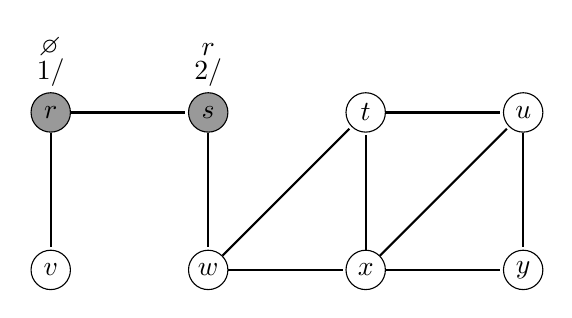
\begin{tikzpicture}[> = stealth,  shorten > = 1pt,   auto,   node distance = 1.5cm]
            \tikzstyle{vertex}=[circle, draw, inner sep=0pt, minimum size=5mm]
    
                % Nós
                \node[vertex, fill=gray!80] (r) at (0,0) {$r$};
                \node[vertex, fill=gray!80] (s) at (2,0) {$s$};
                \node[vertex] (t) at (4,0) {$t$};
                \node[vertex] (u) at (6,0) {$u$};
                \node[vertex] (v) at (0,-2) {$v$};
                \node[vertex] (w) at (2,-2) {$w$};
                \node[vertex] (x) at (4,-2) {$x$};
                \node[vertex] (y) at (6,-2) {$y$};
                
                % Arestas
                \draw[-,thick] (r) -- (v);
                \draw[-,thick] (r) -- (s);
                \draw[-,thick] (s) -- (w);
                \draw[-,thick] (w) -- (t);
                \draw[-,thick] (w) -- (x);
                \draw[-,thick] (x) -- (y);
                \draw[-,thick] (x) -- (u);
                \draw[-,thick] (x) -- (t);
                \draw[-,thick] (t) -- (u);
                \draw[-,thick] (u) -- (y);

                \node at (r) [above=.6cm] {$\diameter$};
                \node at (r) [above=.2cm] {$1\slash$};   
                
                \node at (s) [above=.6cm] {$r$};
                \node at (s) [above=.2cm] {$2\slash$};

                % \node at (x) [below=.15cm] {$cor = P$};
                % \node at (x) [below=.5cm] {$\pi = u$};

                % \node at (x) [below=.15cm] {$cor = P$};
                % \node at (x) [below=.5cm] {$\pi = u$};
                % \node at (x) [below=.75cm] {$d = 1$};
                % \node at (u) [above=.75cm] {$cor = C$};
                % \node at (u) [above=.45cm] {$\pi = \diameter$};
                % \node at (u) [above=.15cm] {$d = 0$};
        \end{tikzpicture}
        \caption{}
    \end{subfigure}
    \\

    \begin{subfigure}{\textwidth}
        \centering
        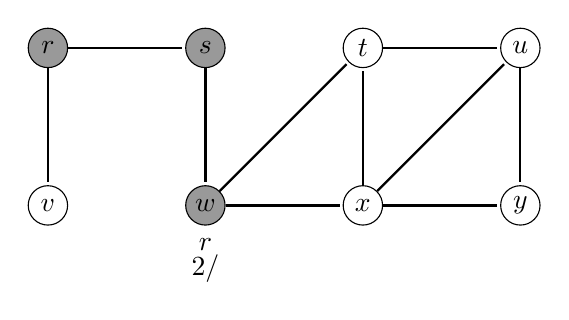
\begin{tikzpicture}[> = stealth,  shorten > = 1pt,   auto,   node distance = 1.5cm]
            \tikzstyle{vertex}=[circle, draw, inner sep=0pt, minimum size=5mm]
    
                % Nós
                \node[vertex, fill=gray!80] (r) at (0,0) {$r$};
                \node[vertex, fill=gray!80] (s) at (2,0) {$s$};
                \node[vertex] (t) at (4,0) {$t$};
                \node[vertex] (u) at (6,0) {$u$};
                \node[vertex] (v) at (0,-2) {$v$};
                \node[vertex, fill=gray!80] (w) at (2,-2) {$w$};
                \node[vertex] (x) at (4,-2) {$x$};
                \node[vertex] (y) at (6,-2) {$y$};
                
                % Arestas
                \draw[-,thick] (r) -- (v);
                \draw[-,thick] (r) -- (s);
                \draw[-,thick] (s) -- (w);
                \draw[-,thick] (w) -- (t);
                \draw[-,thick] (w) -- (x);
                \draw[-,thick] (x) -- (y);
                \draw[-,thick] (x) -- (u);
                \draw[-,thick] (x) -- (t);
                \draw[-,thick] (t) -- (u);
                \draw[-,thick] (u) -- (y);

                
                \node at (w) [below=.3cm] {$r$};
                \node at (w) [below=.5cm] {$2\slash$};

                % \node at (x) [below=.15cm] {$cor = P$};
                % \node at (x) [below=.5cm] {$\pi = u$};
        \end{tikzpicture}
        \caption{}
    \end{subfigure}
    \\

    \begin{subfigure}{\textwidth}
        \centering
        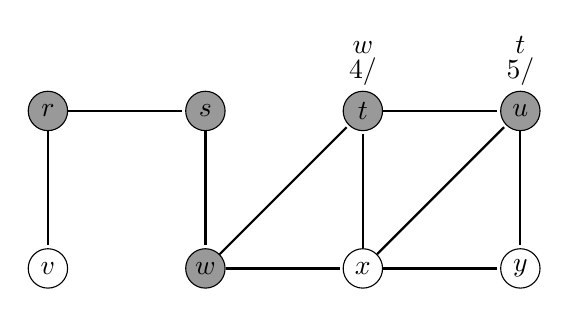
\begin{tikzpicture}[> = stealth,  shorten > = 1pt,   auto,   node distance = 1.5cm]
            \tikzstyle{vertex}=[circle, draw, inner sep=0pt, minimum size=5mm]
    
                % Nós
                \node[vertex, fill=gray!80] (r) at (0,0) {$r$};
                \node[vertex, fill=gray!80] (s) at (2,0) {$s$};
                \node[vertex, fill=gray!80] (t) at (4,0) {$t$};
                \node[vertex, fill=gray!80] (u) at (6,0) {$u$};
                \node[vertex] (v) at (0,-2) {$v$};
                \node[vertex, fill=gray!80] (w) at (2,-2) {$w$};
                \node[vertex] (x) at (4,-2) {$x$};
                \node[vertex] (y) at (6,-2) {$y$};
                
                % Arestas
                \draw[-,thick] (r) -- (v);
                \draw[-,thick] (r) -- (s);
                \draw[-,thick] (s) -- (w);
                \draw[-,thick] (w) -- (t);
                \draw[-,thick] (w) -- (x);
                \draw[-,thick] (x) -- (y);
                \draw[-,thick] (x) -- (u);
                \draw[-,thick] (x) -- (t);
                \draw[-,thick] (t) -- (u);
                \draw[-,thick] (u) -- (y);
                
                \node at (t) [above=.6cm] {$w$};
                \node at (t) [above=.2cm] {$4\slash$};   
                \node at (u) [above=.6cm] {$t$};
                \node at (u) [above=.2cm] {$5\slash$};   
        \end{tikzpicture}
        \caption{}
    \end{subfigure}

\end{figure}
\clearpage
\begin{figure}[H]\ContinuedFloat

    \begin{subfigure}{\textwidth}
        \centering
        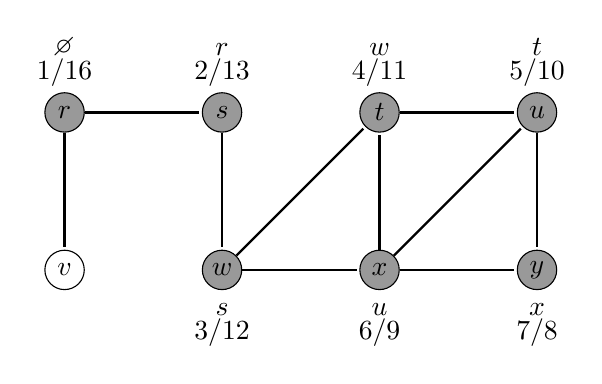
\begin{tikzpicture}[> = stealth,  shorten > = 1pt,   auto,   node distance = 1.5cm]
            \tikzstyle{vertex}=[circle, draw, inner sep=0pt, minimum size=5mm]
    
                % Nós
                \node[vertex, fill=gray!80] (r) at (0,0) {$r$};
                \node[vertex, fill=gray!80] (s) at (2,0) {$s$};
                \node[vertex, fill=gray!80] (t) at (4,0) {$t$};
                \node[vertex, fill=gray!80] (u) at (6,0) {$u$};
                \node[vertex] (v) at (0,-2) {$v$};
                \node[vertex, fill=gray!80] (w) at (2,-2) {$w$};
                \node[vertex, fill=gray!80] (x) at (4,-2) {$x$};
                \node[vertex, fill=gray!80] (y) at (6,-2) {$y$};
                
                % Arestas
                \draw[-,thick] (r) -- (v);
                \draw[-,thick] (r) -- (s);
                \draw[-,thick] (s) -- (w);
                \draw[-,thick] (w) -- (t);
                \draw[-,thick] (w) -- (x);
                \draw[-,thick] (x) -- (y);
                \draw[-,thick] (x) -- (u);
                \draw[-,thick] (x) -- (t);
                \draw[-,thick] (t) -- (u);
                \draw[-,thick] (u) -- (y);

                \node at (r) [above=.6cm] {$\diameter$};
                \node at (r) [above=.2cm] {$1\slash16$};   
                \node at (s) [above=.6cm] {$r$};
                \node at (s) [above=.2cm] {$2\slash13$};   
                \node at (t) [above=.6cm] {$w$};
                \node at (t) [above=.2cm] {$4\slash11$};   
                \node at (u) [above=.6cm] {$t$};
                \node at (u) [above=.2cm] {$5\slash10$};   
                \node at (w) [below=.3cm] {$s$};
                \node at (w) [below=.5cm] {$3\slash12$};
                \node at (x) [below=.3cm] {$u$};
                \node at (x) [below=.5cm] {$6\slash9$};
                \node at (y) [below=.3cm] {$x$};
                \node at (y) [below=.5cm] {$7\slash8$};
                
        \end{tikzpicture}
        \caption{}
    \end{subfigure}
    \\

    \begin{subfigure}{\textwidth}
        \centering
        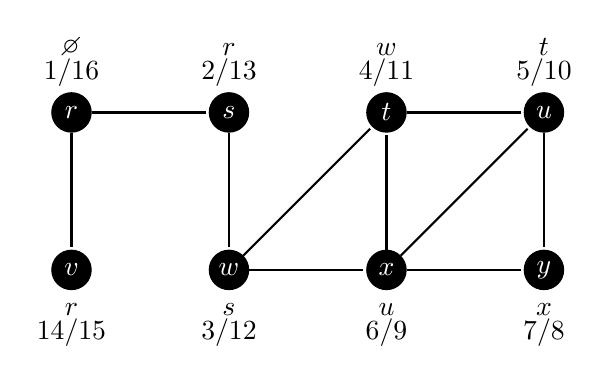
\begin{tikzpicture}[> = stealth,  shorten > = 1pt,   auto,   node distance = 1.5cm]
            \tikzstyle{vertex}=[circle, draw, inner sep=0pt, minimum size=5mm]
    
                % Nós
                \node[vertex, fill=black, text=white] (r) at (0,0) {$r$};
                \node[vertex, fill=black, text=white] (s) at (2,0) {$s$};
                \node[vertex, fill=black, text=white] (t) at (4,0) {$t$};
                \node[vertex, fill=black, text=white] (u) at (6,0) {$u$};
                \node[vertex, fill=black, text=white] (v) at (0,-2) {$v$};
                \node[vertex, fill=black, text=white] (w) at (2,-2) {$w$};
                \node[vertex, fill=black, text=white] (x) at (4,-2) {$x$};
                \node[vertex, fill=black, text=white] (y) at (6,-2) {$y$};
                
                % Arestas
                \draw[-,thick] (r) -- (v);
                \draw[-,thick] (r) -- (s);
                \draw[-,thick] (s) -- (w);
                \draw[-,thick] (w) -- (t);
                \draw[-,thick] (w) -- (x);
                \draw[-,thick] (x) -- (y);
                \draw[-,thick] (x) -- (u);
                \draw[-,thick] (x) -- (t);
                \draw[-,thick] (t) -- (u);
                \draw[-,thick] (u) -- (y);

                \node at (r) [above=.6cm] {$\diameter$};
                \node at (r) [above=.2cm] {$1\slash16$};   
                \node at (s) [above=.6cm] {$r$};
                \node at (s) [above=.2cm] {$2\slash13$};   
                \node at (t) [above=.6cm] {$w$};
                \node at (t) [above=.2cm] {$4\slash11$};   
                \node at (u) [above=.6cm] {$t$};
                \node at (u) [above=.2cm] {$5\slash10$};   
                \node at (v) [below=.3cm] {$r$};
                \node at (v) [below=.5cm] {$14\slash15$};
                \node at (w) [below=.3cm] {$s$};
                \node at (w) [below=.5cm] {$3\slash12$};
                \node at (x) [below=.3cm] {$u$};
                \node at (x) [below=.5cm] {$6\slash9$};
                \node at (y) [below=.3cm] {$x$};
                \node at (y) [below=.5cm] {$7\slash8$};
        \end{tikzpicture}
        \caption{}
    \end{subfigure}

\end{figure}


\section{} % 6
    O grafo tem ciclo quando o vértice inicial percorre um caminho e no final do caminho está o vértice inicial já descoberto, no caso da questão é o caminho $\{a,b,e,c,a\}$. Se pegar outra fonte acontece a mesma coisa, tipo o caminho $\{a,c,d,a\}$
    
    Nesse caso, é usando a busca em profundidade, onde teria que verificar todos os vértices adjacentes atingiveis a partir da fonte, pegando como exemplo o $\{a,b,e,c,a\}$. Quando seguir esse caminho o vértice a já vá estar descoberto (ou seja, pintado de cinza) e aí se constaria o ciclo.

\section{} % 7
    A ordenação topológica em um grafo é uma disposição linear dos seus vértices de tal forma que para cada aresta direcionada, o nó de origem aparece antes do nó de destino na sequência. Essa ordenação ajuda a determinar a sequência correta de execução de tarefas, garantindo que todas as depedências sejam atendidas. 

    \begin{flalign*}
        \text{Ordem topológica: } \{a, b, d, c, e\}
    \end{flalign*}

        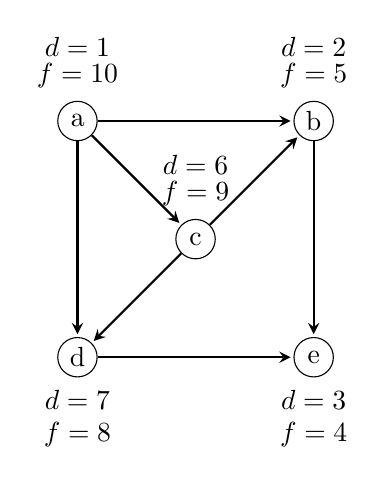
\begin{tikzpicture} [> = stealth,  shorten > = 1pt,   auto,   node distance = 1.5cm]
            % Estilo para os nós
            \tikzstyle{vertex}=[circle, draw, inner sep=0pt, minimum size=5mm]
            
            % Nós
            \node[vertex] (a) at (0,0) {a};
            \node[vertex] (b) at (3,0) {b};
            \node[vertex] (c) at (1.5,-1.5) {c};            
            \node[vertex] (d) at (0,-3) {d};
            \node[vertex] (e) at (3,-3) {e};
            
            % Arestas
            \draw[->,thick] (a) -> (b);
            \draw[->,thick] (a) -> (c);
            \draw[->,thick] (a) -> (d);
            \draw[->,thick] (b) -> (e);
            \draw[->,thick] (c) -> (b);
            \draw[->,thick] (c) -> (d);
            \draw[->,thick] (d) -> (e);
            
            % Anotações
            \node at (a) [above=0.7cm] {$d = 1$};
            \node at (a) [above=0.3cm] {$f = 10$};
            \node at (b) [above=0.7cm] {$d = 2$};
            \node at (b) [above=0.3cm] {$f = 5$};
            \node at (c) [above=0.7cm] {$d = 6$};
            \node at (c) [above=0.3cm] {$f = 9$};
            \node at (d) [below=.3cm] {$d = 7$};
            \node at (d) [below=.7cm] {$f = 8$};
            \node at (e) [below=.3cm] {$d = 3$};
            \node at (e) [below=.7cm] {$f = 4$};
        \end{tikzpicture}

\section{} % 8
\begin{python}
from collections import deque

def bfs(grafo: dict, fonte: str, alvo: str) -> list:
    pais: dict = {fonte: None}
    # Cria fila com o primeiro elemento
    fila: deque = deque([fonte])
    while fila:
        # Remove o primeiro elemento da fila
        vertice: str = fila.popleft()
        for vizinho in grafo[vertice]:
            vizinho: str
            if vizinho not in pais:
                # Se o vizinho nao estiver no dicionario de pais
                # Adiciona o vizinho no dicionario de pais
                pais[vizinho] = vertice
                fila.append(vizinho)
                if vertice == alvo:
                    # Se o node atual for o alvo, para a busca
                    # retorna o caminho
                    break

    caminho = [alvo]
    while pais[alvo] is not None:
        caminho.insert(0, pais[alvo])
        alvo = pais[alvo]

    return caminho
\end{python}
\href{https://github.com/aejunior/bsi-ed-ii/blob/master/src/search/bfs.py}{\faGithub}

\section{} % 9
\begin{python}
def dfs(grafo: dict, inicio: str, alvo: str):
    visitado, pilha = [], [inicio]
    caminho: list = []  # Cria lista para armazenar o caminho
    while pilha:
        vertice = pilha.pop()
        if vertice not in visitado:
            visitado.append(vertice)
            caminho.append(vertice)  # Adiciona o vertice ao caminho
            if vertice == alvo:
                return caminho
            pilha.extend(set(grafo[vertice]) - set(visitado)) 
    return []  # Se nao encontra, retorna lista vazia
\end{python}
\href{https://github.com/aejunior/bsi-ed-ii/blob/master/src/search/dfs.py}{\faGithub}

\end{document}